\documentclass[tikz,border=8pt]{standalone}
\usetikzlibrary{arrows.meta,calc}
\begin{document}
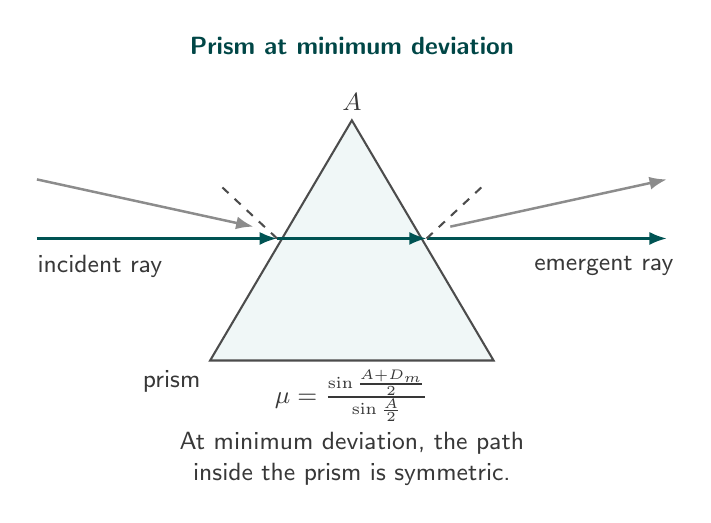
\begin{tikzpicture}[
  ray/.style={-{Latex[length=2.2mm]},draw=teal!65!black,line width=0.9pt},
  line/.style={draw=black!70,line width=0.75pt},
  label/.style={font=\sffamily\small,text=black!78},
  title/.style={font=\sffamily\bfseries\small,text=teal!55!black},
]
\node[title] at (0,3.0) {Prism at minimum deviation};
\coordinate (A) at (0,2.05);
\coordinate (B) at (-1.8,-1.0);
\coordinate (C) at (1.8,-1.0);
\draw[line,fill=teal!6] (A)--(B)--(C)--cycle;
\node[label,above] at (A) {$A$};
\node[label,below left] at (B) {prism};
\draw[ray] (-4,0.55)--(-0.95,0.55);
\draw[ray] (-0.95,0.55)--(0.95,0.55);
\draw[ray] (0.95,0.55)--(4,0.55);
\draw[line,dashed] (-0.95,0.55)--(-1.7,1.25);
\draw[line,dashed] (0.95,0.55)--(1.7,1.25);
\draw[ray,black!45] (-4,1.3)--(-1.25,0.7);
\draw[ray,black!45] (1.25,0.7)--(4,1.3);
\node[label] at (-3.2,0.2) {incident ray};
\node[label] at (3.2,0.2) {emergent ray};
\node[label] at (0,-1.45) {$\mu=\frac{\sin\frac{A+D_m}{2}}{\sin\frac{A}{2}}$};
\node[label,align=center,text width=8cm] at (0,-2.25) {At minimum deviation, the path inside the prism is symmetric.};
\end{tikzpicture}
\end{document}
